\documentclass[
  bibliography=totoc,     % Literatur im Inhaltsverzeichnis
  captions=tableheading,  % Tabellenüberschriften
  titlepage=firstiscover, % Titelseite ist Deckblatt
]{scrartcl}

\usepackage{fixltx2e}
\usepackage[aux]{rerunfilecheck}

\usepackage{polyglossia}
\setmainlanguage{german}

\usepackage{amsmath}
\usepackage{amssymb}
\usepackage{mathtools}

\usepackage{fontspec}
\defaultfontfeatures{Ligatures=TeX}

\usepackage[
  math-style=ISO,
  bold-style=ISO,
  sans-style=italic,
  nabla=upright,
  partial=upright,
]{unicode-math}

\usepackage[autostyle]{csquotes}

\usepackage[
  locale=DE,                   % deutsche Einstellungen
  separate-uncertainty=true,   % Immer Fehler mit \pm
  per-mode=symbol-or-fraction, % m/s im Text, sonst Brüche
]{siunitx}

\usepackage[version=3]{mhchem}

\usepackage{xfrac}

\usepackage[section, below]{placeins}
\usepackage[
  labelfont=bf,        % Tabelle x: Abbildung y: ist jetzt fett
  font=small,          % Schrift etwas kleiner als Dokument
  width=0.9\textwidth, % maximale Breite einer Caption schmaler
]{caption}
\usepackage{subcaption}
\usepackage{graphicx}
\usepackage{grffile}

\usepackage{float}
\floatplacement{figure}{htbp}
\floatplacement{table}{htbp}

\usepackage{booktabs}

\usepackage[
  unicode,
  pdfusetitle,    % Titel, Autoren und Datum als PDF-Attribute
  pdfcreator={},  % PDF-Attribute säubern
  pdfproducer={}, % "
]{hyperref}
\usepackage{bookmark}
\usepackage[shortcuts]{extdash}


\title{Entwicklung eines mobil lauffähigen microblog-Systems mit flask und
CouchDB}
\subtitle{Ein Projekt der PeP et Al. Sommerakademie 2014}
\date{24. -- 31. August 2014}

\author{
    Kevin Heinicke
}

\begin{document}

\maketitle
\tableofcontents

\section{Einleitung}
Aus einer ersten Idee, ein mobiles, drahtloses Netzwerk auf einem RaspberryPi
einzurichten, um damit selbst auf den höchsten österreicher Bergen eine
gewisse digitale Grundversorgung bereitzustellen ist schnell das Projekt
eines minimalistischen Blogs entstanden.
Hiermit sollte eine etwas andere Perspektive SoAk-Dokumentation ermöglicht
werden, indem jeder Teilnehmer jederzeit seine Eindrücke mitteilen kann.

\section{Technische Umsetzung}
Um die Idee zu realisieren wird ein RaspberryPi-Computer verwendet, der mit
Hilfe eines USB-Akkus und eines WLAN-Sticks als mobiler Accesspoint dient.
Eine erste Abschätzung für die Laufzeit des Systems bei Akkubetrieb lässt
eine dauerhafte Nutzung für etwa 7 Stunden erwarten.
\begin{figure}
  \centering
  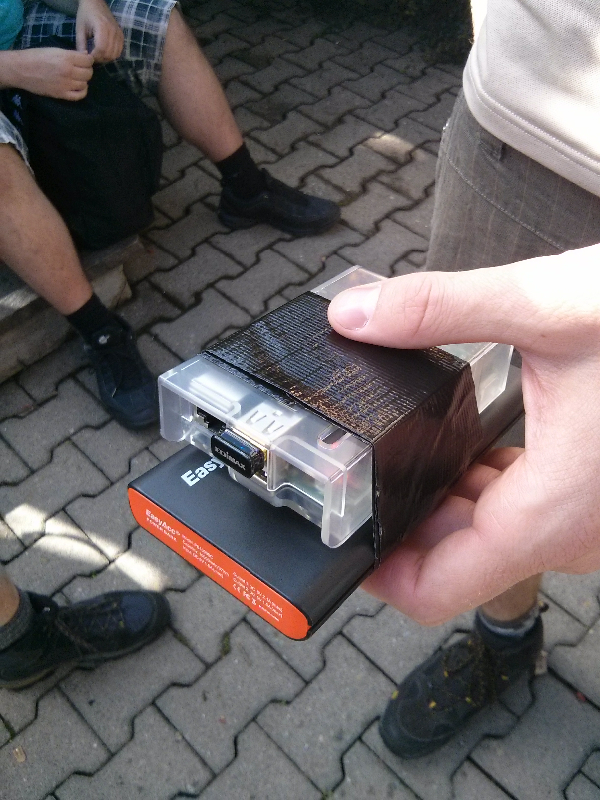
\includegraphics[width=0.5\linewidth]{images/raspi1.jpg}
  \caption{Mobiler Aufbau des RaspberryPis mit angeschlossenem Akku
  und WLAN-Dongle.}
  \label{fig:raspi}
\end{figure}

Das Blogsystem beruht auf dem python-Framework flask, welches eine
ausgesprochen simple Erstellung einer Website mit allen wichtigen Funktionen
bietet.
Die flask-app wird maßgeblich zur Kommunikation mit der CouchDB-Datenbank
gentzt, wobei es sich um eine objektorientierte Datenbank handelt.
Der Quellcode des Systems ist auf
\href{https://github.com/bixel/microblog}{github.com} zugänglich.
Die Nutzung einer objektorientierten Datenbank ermöglicht eine besonders
freie Entwicklung, was für den nachträglichen Einbau von Zusatzfunktionen
ausgesprochen hilfreich ist.

Das erste Ziel des Systems ist die Speicherung von Text- und Bildbeiträgen
von verschiedenen Nutzern, sowie die chronologische Wiedergabe dieser Beiträge.
Um die Ressourcenanforderungen an den RaspberryPi zu verkleinern,
stellt sich das CSS- und JavaScript-Framework bootstrap als sehr hilfreich
heraus, da eine optisch ansprechende Basiselemente für eine Interaktive
Webapp, wie dem microblog bietet.

\section{Ergebnisse}
Die Nutzung des microblog-Systems stellt sich als voller Erfolg heraus.
Über die Dauer der Reise wurden insgesamt 208 Beiträge verfasst.
Der Erfolgreichste Beitrag war mit insgesamt \num{8} Likes ein Bild
des Teams Astrofotografie.
Besonders beliebt waren ebenfalls Aufnahmen aus dem Bereich
\enquote{Speisen und Getränke}.
Während der großen Wanderung zur Mittagsspitze wurden insgesamt \num{32}
Bilder hochgeladen und der Akku des Systems verlor in dieser Zeit
lediglich etwa \SI{50}{\percent} der Ladung.

\section{Probleme und Verbesserungsmöglichkeiten}
Nach der Umsetzung der ersten Mindestanforderungen in einer
Entwicklungsumgebung stellt sich die Installation auf dem RaspberryPi als
langwierige Problemsuche dar.
Es muss zunächst einige Erfahrung in der Einrichtung der genutzten Software auf
einem Minicomputer, wie dem RaspberryPi gesammelt werden, bevor das System auch
zuverlässig arbeitet.

Noch während der Anreise wurden dem System weitere Features, wie eine
\enquote{Likefunktion} und der Möglichkeit, Beiträge zu verstecken
eingearbeitet.
Insgesamt stellte sich jedoch die Pflege des Systems bei laufendem Betrieb als
zu zeitintensiv für eine solche Reise heraus, weshalb die unzählichen
-- teilweise guten, teilweise spaßigen -- Nachfragen nach neuen Funktionen
auf einen späteren Zeitpunkt verschoben werden musste.

Nach Ankunft zeigte sich zudem, dass die Leistung des RaspberryPi nach einiger
Nutzung des Systems an dessen Grenzen stoß. Besonders die WLAN-Funktionalität
war für die Räumlichkeiten nicht ausreichend.
\end{document}
